%!TEX TS-program = pdflatex
\documentclass[ngerman]{beamer}

\usepackage[T1]{fontenc}
\usepackage{babel}
\usepackage{csquotes}
\setbeamertemplate{navigation symbols}{}

\setbeamercolor{block body alerted}{bg=alerted text.fg!10}
\setbeamercolor{block title alerted}{bg=alerted text.fg!20}
\setbeamercolor{block body}{bg=structure!10}
\setbeamercolor{block title}{bg=structure!20}
\setbeamercolor{block body example}{bg=green!10}
\setbeamercolor{block title example}{bg=green!20}

% https://tex.stackexchange.com/questions/339462/beamer-table-of-content-put-only-the-current-section-and-subsection-at-the-top
\AtBeginSection{%
    \begin{frame}
\begin{center}
        \LARGE\bfseries\tableofcontents[sections=\value{section}]
\end{center}
    \end{frame}
}

\usepackage{xcolor}
\usepackage{listings}
\lstset{upquote=true}



\lstdefinestyle{latex}{basicstyle=\ttfamily,morekeywords={usepackage,varobar,defbeamertemplate,definecolor,setbeamertemplate,usebeamertemplate,usetheme,gettwofromjobname,setbeamercolor,setbeamerfont,tiny,addtobeamertemplate,itshape,sffamily,twemoji}}

\lstdefinestyle{latexf}{style=latex, language=[LaTeX]TeX,
basicstyle=\ttfamily\footnotesize}

\lstdefinestyle{Python}{language=Python,basicstyle=\ttfamily\footnotesize,morekeywords={read_csv}}

\usepackage{attachfile}
\newcommand{\ta}[1]{\textattachfile[color=1 0 0]{#1}{Code}}

\newcommand{\pypy}[2]{\lstinputlisting[language={Python},caption={#1 \ta{#2}}]{#2}}

\makeatletter
\lstdefinestyle{ausgabe}{
  basicstyle=\ttfamily\scriptsize,%
  backgroundcolor=\color{lightgray}%
}
\makeatother

\lstnewenvironment{ausgabe}{\lstset{style=ausgabe}}{} 

\definecolor{colBack}{rgb}{1,1,0.9}
\definecolor{colKeys}{rgb}{0,0,1}
\definecolor{colIdentifier}{rgb}{0,0,0}
\definecolor{colComments}{rgb}{1,0,0}
\definecolor{colString}{rgb}{0,0.5,0}

\lstset{literate=%
    {Ö}{{\"O}}1
    {Ä}{{\"A}}1
    {Ü}{{\"U}}1
    {ß}{{\ss}}1
    {ü}{{\"u}}1
    {ä}{{\"a}}1
    {ö}{{\"o}}1
    {~}{{\textasciitilde}}1
}


\lstset{%
    float=hbp,%
    basicstyle=\ttfamily\footnotesize, %
    identifierstyle=\color{colIdentifier}, %
    keywordstyle=\color{colKeys}, %
    stringstyle=\color{colString}, %
    commentstyle=\color{colComments}, %
    columns=flexible, %
    tabsize=2, %
    frame=single, %
    extendedchars=true, %
    showspaces=false, %
    showstringspaces=false, %
    numbers=left, %
    numberstyle=\tiny, %
    breaklines=true, %
    backgroundcolor=\color{colBack}, %
    breakautoindent=true, %
    captionpos=b,%
    language={Python},
    morekeywords={copyfile,write,unlink}
}


\usepackage[T1]{fontenc}

\newcommand{\bild}[1]{\fbox{\includegraphics[width=0.2\textwidth]{Presentation-AnnArbor-#1}}}

\author{Uwe Ziegenhagen}
\title{Python \& pandas}
\subtitle{A one day course}
\institute{\url{github.com/UweZiegenhagen/OneDayPythonPandasCourse}}
\date{Cologne, \today}


\begin{document}

\begin{frame}

\maketitle

\end{frame}

\section{Introduction}

\begin{frame}[fragile]
\frametitle{Why Python/pandas?}

\begin{itemize}
	\item You \textit{have} a CSV-file with semicolon as column separator and comma as decimal separator
	\item You \textit{need} a CSV-file with comma as column separator and dot as decimal separator
\end{itemize}

\begin{lstlisting}
import pandas as pd

df = pd.read_csv('myfile.csv', sep=';', decimal = ',')
df = pd.to_csv('myfile.csv', sep=';', decimal = ',')
\end{lstlisting}


\end{frame}

\begin{frame}
\frametitle{Limits of this Course}

\begin{itemize}
\item It is not a \textit{full} course, we would need a whole week for this.
\item We will skip many interesting things (that you do not necessarily need for your job)
\item Goal: Teach you enough Python to a) read and b) understand Python-Code and c) write smaller programs relevant for your job 
\end{itemize}
\end{frame}



\begin{frame}

\tableofcontents

\end{frame}


\begin{frame}
\frametitle{Python}

\begin{itemize}
	\item Invented by Guido van Rossum at the \enquote{Centrum Wiskunde \& Informatica} in Amsterdam as successor for the teaching language ABC
	\item Current version is 3.11
	\item For a long time, Python 3.x and Python 2.7 existed together
	\item Python 2.7 support expired in 2019:
	\item How to spot 2.7 code: $\rightarrow$ \texttt{print 'hello'} instead of \texttt{print('hello')}
\end{itemize}

\end{frame}

\begin{frame}
\frametitle{Python versus Java \& C}

Python code is often much slower than C or Java but\ldots

\begin{itemize}
\item the implementation time for Python is way faster
\item speeds only matters sometimes, not always
\item many computing-intensive Python modules use\newline C/C++ modules \enquote{under the hood}
\item bad C-Code is slower than good Python-code
\end{itemize}
\end{frame}


\begin{frame}
\frametitle{pandas}

\begin{itemize}
	\item A Python library for data wrangling and management
	\item Invented by Wes McKinney during his time at AQR Capital Management
	\item In his own words:
\enquote{I tell them that it enables people to analyze and work with data who are not expert computer scientists,} he says. \enquote{You still have to write code, but it’s making the code intuitive and accessible. It helps people move beyond just using Excel for data analysis.}\footnote{\url{qz.com/1126615/the-story-of-the-most-important-tool-in-data-science/}}
\end{itemize}

\end{frame}

\section{Python}

\begin{frame}
\frametitle{Spyder}

\begin{itemize}
	\item We will use the Spyder5 IDE with Python 3.9.9, make sure it is installed
\end{itemize}

\begin{center}
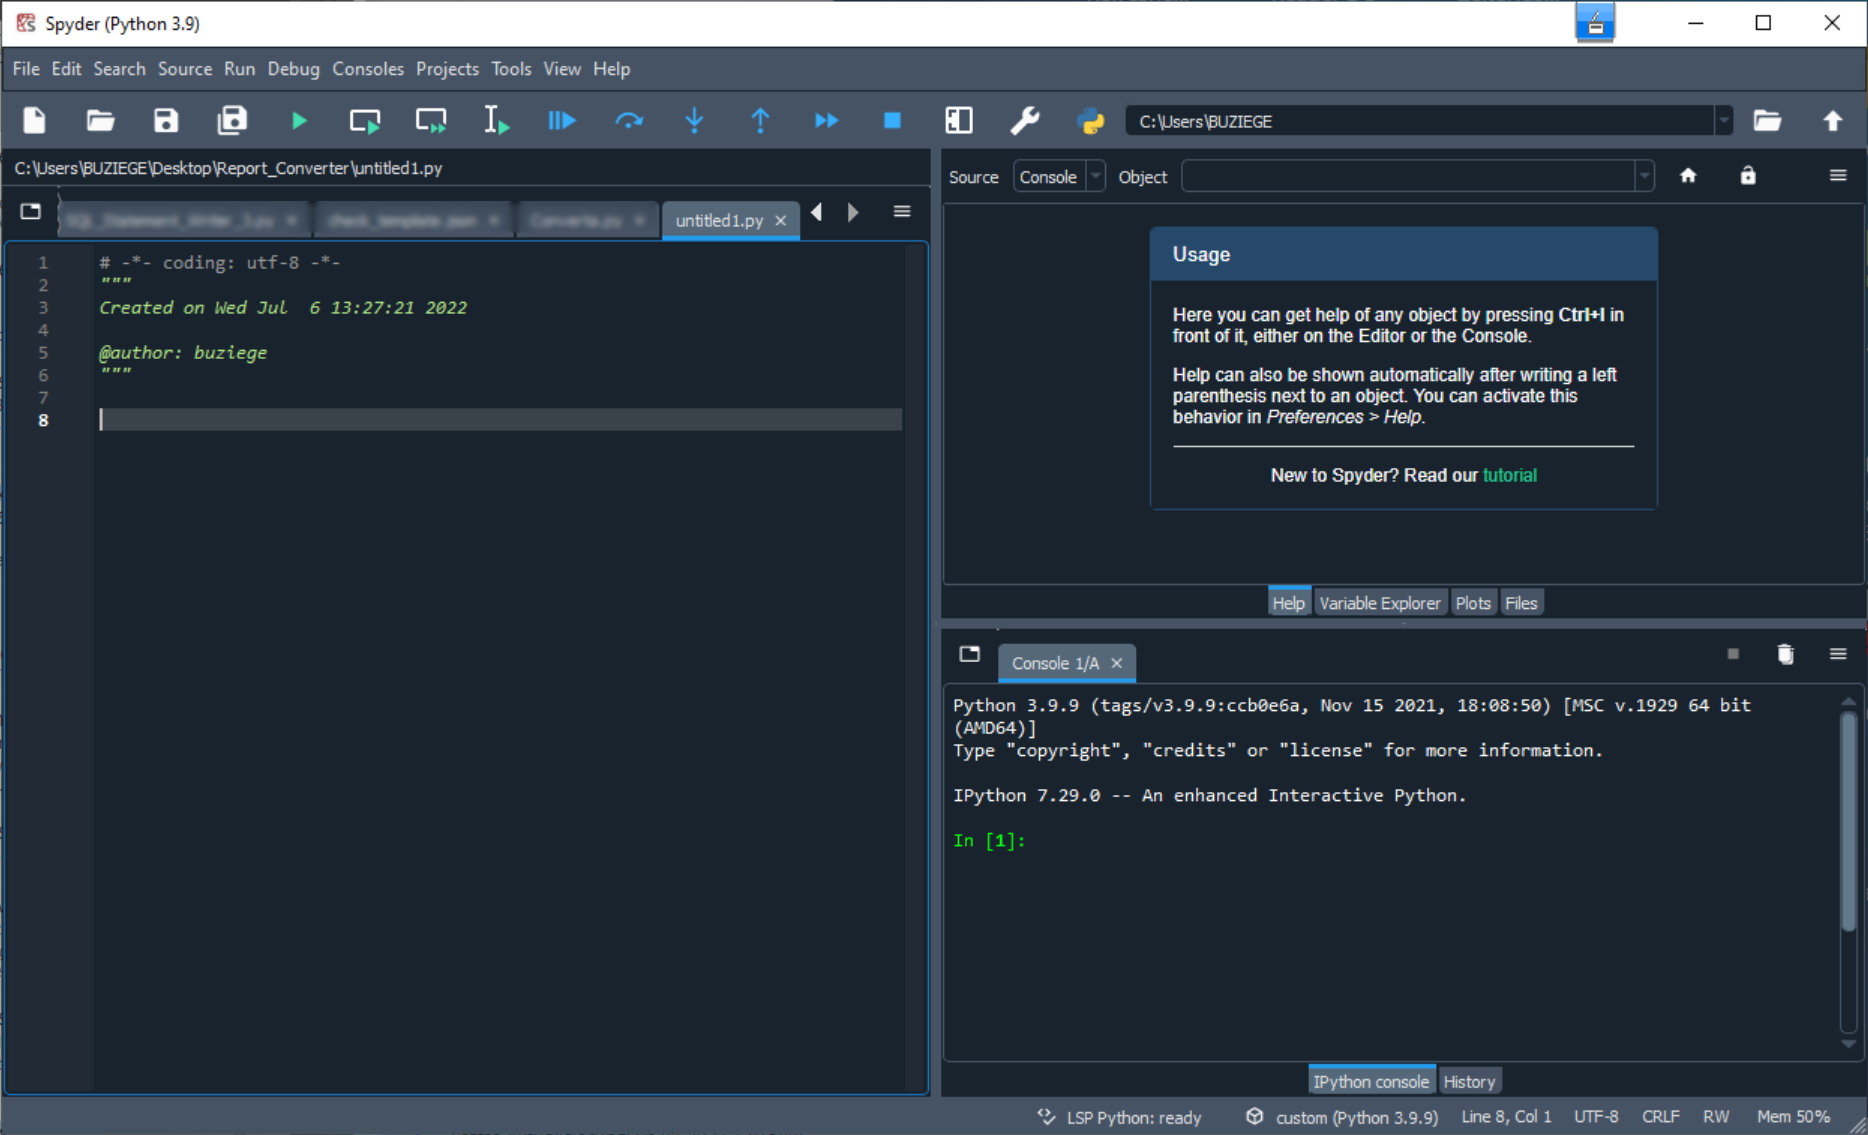
\includegraphics[width=\textwidth]{Pictures/Spyder5}
\end{center}

\end{frame}

\begin{frame}[fragile]
\frametitle{Python as a Calculator}

\begin{itemize}
\item Spyder5 runs an IPython kernel, this runs our programs
\item We can also use it as a calculator
\end{itemize}

\begin{lstlisting}[style=Python]
In [1]: 4*5.4
Out[1]: 21.6

In [2]: 4/12
Out[2]: 0.3333333333333333

In [3]: _*3
Out[3]: 1.0

'hello'
Out[4]: 'hello'
\end{lstlisting}

\end{frame}


\begin{frame}[fragile]
\frametitle{Python as a Calculator}

\begin{lstlisting}[style=Python]

In [1]: 4%2
Out[1]: 0

In [2]: 5%2 # Modulo
Out[2]: 1

In [3]: 3**3
Out[3]: 27

In [4]: 5//2
Out[4]: 2
\end{lstlisting}

\end{frame}

\begin{frame}
\frametitle{Priority of Operators}

\begin{itemize}
\item Round brackets have highest priority
\item followed by Power
\item followed by multiplication and division
\item followed by addition and substraction
\end{itemize}

\begin{block}{TODO4U:}
$\Rightarrow$ Solve exercise sheet 1!
\end{block}

\end{frame}

\begin{frame}[fragile]
\frametitle{Basic Input \& Output}

\lstinputlisting[style=Python]{Codes/Basic_IO.py}

\begin{itemize}
	\item \lstinline[style=Python]{input()} only reads strings	
	\item If you need a number, you need to convert it
	\item there are better ways than \lstinline[style=Python]{print()} for logging, but it works\ldots 
	\item f-Strings (last row) are recommended for mixed output!
	\end{itemize}
\end{frame}

\begin{frame}
\frametitle{Rules for Variables}

\begin{itemize}
\item must start with a letter or \textunderscore
\item Case-sensitivity: 'A' is not 'a'
\item Recommendation: small letters
\item Let them speak for themselves: 'diameter' is good, 'd' is bad 
\end{itemize}
\end{frame}


\begin{frame}
\frametitle{Reserved Keywords}

The following  keywords are reserviert and must not be used for variables' names.

\begin{center}
\begin{tabular}{p{0.15\textwidth}p{0.15\textwidth}p{0.15\textwidth}p{0.15\textwidth}p{0.15\textwidth}}
and	&	as	&	assert	&	break	&	class	\\
continue	&	def	&	del	&	elif	&	else	\\
except	&	False	&	finally	&	for	&	from	\\
global	&	if	&	import	&	in	&	is	\\
lambda	&	None	&	nonlocal	&	not	&	or	\\
pass	&	raise	&	return	&	True	&	try	\\
while	&	with	&	yield	&		&		\\
\end{tabular}
\end{center}
\end{frame}



\subsection{Datentypen}

\begin{frame}
\frametitle{Datentypen}


\begin{itemize}
\item Integer (ganze Zahlen)
\item Float (Fließkommazahlen)
\item Zeichenketten
\item Boolesche Werte
\item Komplexe Zahlen
\end{itemize}
\end{frame}

\begin{frame}
\frametitle{Integer}


\begin{itemize}
\item unbegrenzte Länge, im Gegensatz zu anderen Sprachen
\item dürfen nicht mit 0 beginnen, wenn es sich um Zahl im Dezimalsystem handeln soll
\item Führende 0 bei Darstellung in Hexadezimal-, Binär- und Oktalsystem:
\begin{description}
\item[\texttt{0b/0B}] Binärzahl
\item[\texttt{0x/0X}] Hexadezimalzahl
\item[\texttt{0o/0O}] Oktalzahl 
\end{description}
\item Funktionen \texttt{hex()}, \texttt{bin()}, \texttt{oct()} für Umwandlung in passenden String
\item Interne Darstellung als Dezimalzahl
\end{itemize}
\end{frame}

\begin{frame}
\frametitle{Float}

\begin{itemize}
	\item Fließkommazahlen
	\item \texttt{3.1415927}
	\item \texttt{3.1e8}
	\item Hinweis: Nicht jede Fließkommazahl kann genau dargestellt werden (\enquote{Floating-Point Arithmetic}) 
	\item \url{docs.python.org/3/tutorial/floatingpoint.html}
\end{itemize}
\end{frame}

\begin{frame}[containsverbatim]
\frametitle{Strings}

\begin{itemize}
\item Doppelte oder einfache Anführungsstriche
\item Mehrzeilige Strings:

\begin{itemize}
	\item Dreifache doppelte oder einfache Anführungsstriche
	\item Alternativ Backslash am Ende der Zeile 
\end{itemize}

\item Zahlreiche Funktionen zur String-Verarbeitung, Details später
\end{itemize}


\begin{lstlisting}[language={Python}]
a = "Ich bin ein String"

b = 'Ich auch'

c = """Ich bin auch
ein String"""
# 'Ich bin auch\nein String'
\end{lstlisting}


\end{frame}

\begin{frame}[containsverbatim]
\frametitle{Boolesche Werte}

\begin{itemize}
	\item Benannt nach George Boole
	\item 1854: \enquote{An investigation into the Laws of Thought}
	\item Herzstück moderner Computertechnik
	\item Boolesche Operatoren or ($\cup$ ),  and ($\cap$ ), \texttt{not}
\end{itemize}

\begin{lstlisting}[language={Python}]
a = True
b = False 

a == b #False
a or b # True
a and b # False
a and not b # True
not a and b # False
\end{lstlisting}
\end{frame}



\begin{frame}[containsverbatim]
\frametitle{Typumwandlungen}

\begin{itemize}
\item Das Mischen von Strings und Float/Integer erfordert explizite Typumwandlung mittels \lstinline[language={Python}]{str()} Funktion
\item Hinweis: pandas hat dazu \lstinline[morekeywords={astype},language={Python}]{.astype(<Datentyp>)} 
\end{itemize}

\begin{lstlisting}[language={Python}]
>>> a + str(b)
'abc123'
>>> a+str(c)
'abc3.141'
>>> a*str(b)
Traceback (most recent call last):
  File "<stdin>", line 1, in <module>
TypeError: can't multiply sequence by non-int of type 'str'
\end{lstlisting}

%\begin{center}
%\fomh{$\Rightarrow$ Bitte Arbeitsblatt 2 bearbeiten!}
%\end{center}

\end{frame}

\subsection{Funktionen}


\begin{frame}
\frametitle{Funktionen}

\begin{itemize}
\item Bereits bekannte Funktionen:  \lstinline[language={Python}]{id()} ,
\lstinline[language={Python}]{len()} 
und \lstinline[language={Python}]{type()} 
\item Funktion: Benannte Sequenz von Befehlen
\item Zweck: Code kapseln, um mehrfachen Aufruf  zu erleichtern
\item Können Argumente als Input bekommen, können Rückgabewerte zurückgeben
\item Definition einer neuen Funktion:
\begin{itemize}
	\item Namen festlegen
	\item Argumente festlegen
	\item Befehlssequenz festlegen
	\end{itemize}
\end{itemize}
\end{frame}


\begin{frame}
\frametitle{Eingebaute Funktionen}

\begin{tabular}{lllll}
abs	&	delattr	&	hash	&	memoryview	&	set	\\
all	&	dict	&	help	&	min	&	setattr	\\
any	&	dir	&	hex	&	next	&	slice	\\
ascii	&	divmod	&	id	&	object	&	sorted	\\
bin	&	enumerate	&	input	&	oct	&	staticmethod	\\
bool	&	eval	&	int	&	open	&	str	\\
breakpoint	&	exec	&	isinstance	&	ord	&	sum	\\
bytearray	&	filter	&	issubclass	&	pow	&	super	\\
bytes	&	float	&	iter	&	print	&	tuple	\\
callable	&	format	&	len	&	property	&	type	\\
chr	&	frozenset	&	list	&	range	&	vars	\\
classmethod	&	getattr	&	locals	&	repr	&	zip	\\
compile	&	globals	&	map	&	reversed	&	\textunderscore \textunderscore import \textunderscore \textunderscore	\\
complex	&	hasattr	&	max	&	round	&		\\
\end{tabular}
\end{frame}

\begin{frame}
\frametitle{Eingebaute Funktionen I}

* steht für \enquote{vermutlich keine Relevanz in der Vorlesung}

\begin{description}
\item[abs()] Absolutwert einer Zahl
\item[all()] prüft, ob alle Elemente eines iterable True sind*
\item[any()] prüft, ob wenigstens Elemente eines iterable True ist*
\item[ascii()] ASCII Darstellung eines Objekts
\item[bin()] wandelt in Binärzahl um
\item[bool()] gibt Boole'schen Wert für Ausdruck zurück 
\end{description}
\end{frame}

\begin{frame}
\frametitle{Eingebaute Funktionen II}

\begin{description}
\item[breakpoint()] im Debugging genutzt*
\item[bytearray()] erzeugt Array of Bytes*
\item[bytes()] erzeugt neues Byte-Objekt*
\item[callable()] Prüfung, ob Objekt aufrufbar ist*
\item[chr()] Unicode-String-Repräsentation einer Zahl
\item[classmethod()] wandelt Methode in Klassenmethode um*
\end{description}
\end{frame}


\begin{frame}
\frametitle{Eingebaute Funktionen III}

\begin{description}
\item[compile()] übersetzt String in exec-baren Code*
\item[complex()] erzeugt komplexe Zahl*
\item[delattr()] löscht Attribut aus Objekt
\item[dict()] erstellt ein dictionary Objekt
\item[dir()] Variablenliste im aktuellen Scope
\item[divmod()] gibt Tupel aus Integer Division und Rest zurück
\end{description}
\end{frame}


\begin{frame}
\frametitle{Eingebaute Funktionen III}

\begin{description}
\item[enumerate()] erzeugte Liste von Zahl, Item aus Iterables
\item[eval()] parst und führt String-Ausdruck aus
\item[exec()] führt dynamisch erzeugten Code aus
\item[filter()] genutzt in funktionaler Programmierung
\item[float()] erstellt float aus Zahl oder String
\item[format()] erstellt formatierten String
\end{description}
\end{frame}


\begin{frame}
\frametitle{Eingebaute Funktionen IV}

\begin{description}
\item[frozenset()] erzeugt unmutuable Set*
\item[getattr()] gibt Wert von Attribut eines Objekts zurück
\item[globals()] gibt dict der globalen Symboltabelle zurück
\item[hasattr()] prüft ob Objekt ein Attribut hat
\item[hash()] gibt integer Hash-Wert für Objekt zurück
\item[help()] ruft die Hilfe auf
\end{description}
\end{frame}


\begin{frame}
\frametitle{Eingebaute Funktionen V}

\begin{description}
\item[hex()] Hexadezimaldarstellung
\item[id()] Gibt die interne ID eines Objekts zurück
\item[input()] liest von der Tastatur einen String
\item[int()] erzeugt integer aus Zahl oder String
\item[isinstance()] prüft, ob Objekt von Typ x ist
\item[issubclass()] prüft, ob Klasse Subklasse von x ist
\end{description}
\end{frame}


\begin{frame}
\frametitle{Eingebaute Funktionen VI}

\begin{description}
\item[iter()] iteriert über Sequenz
\item[len()] Länge eines Objekt
\item[list()] erzeugt Liste
\item[locals()] erzeugt Update für die 
\item[map()] genutzt in funktionaler Programmierung
\item[max()] gibt Maximum zurück
\end{description}
\end{frame}


\begin{frame}
\frametitle{Eingebaute Funktionen VII}

\begin{description}
\item[memoryview()] gibt memoryview eines Objekts wieder*
\item[min()] gibt Minimum zurück
\item[next()] gibt nächstes Objekt von Iterator zurück
\item[object()] gibt neues Objekt zurück*
\item[oct()] Oktaldarstellung einer Zahl*
\item[open()] öffnet Datei zum Lesen/Schreiben
\end{description}
\end{frame}


\begin{frame}
\frametitle{Eingebaute Funktionen VIII}

\begin{description}
\item[ord()] Inverse von chr(), gibt Zahl für Zeichen aus
\item[pow()] analog zu x**y
\item[print()] gibt Objekte aus auf Kommandozeile, in Datei
\item[property()] gibt Property-Attribut aus*
\item[range()] erzeugt eine Zahlenliste
\item[repr()] gibt ASCII-Repräsentation eines Objekts wieder*
\end{description}
\end{frame}


\begin{frame}
\frametitle{Eingebaute Funktionen IX}

\begin{description}
\item[reversed()] gibt umgekehrte Sequence zurück
\item[round()] rundet Zahl
\item[set()] erstellt Menge
\item[setattr()] Gegenstück zu getattr()
\item[slice()] gibt slice-Objekt zurück*
\item[sorted()] gibt sortierte Liste zurück
\end{description}
\end{frame}


\begin{frame}
\frametitle{Eingebaute Funktionen X}

\begin{description}
\item[staticmethod()] wandelt Methode in statische Methode um*
\item[str()] erzeugt String aus Objekt
\item[sum()] berechnet Summe aus 
\item[super()] gibt Proxy-Objekt zurück*
\item[tuple()] erzeugt Tupel aus Iterable
\item[type()] gibt Typ eines Objekts wieder
\end{description}
\end{frame}


\begin{frame}
\frametitle{Eingebaute Funktionen XI}

\begin{description}
\item[vars()] gibt dict-Attribut eines Objekts wider
\item[zip()] aggregiert iterables in einen Iterator
\item[\textunderscore \textunderscore import()\textunderscore \textunderscore] Funktion zum Anpassen von import-Statements*
\end{description}



\end{frame}


\begin{frame}[containsverbatim]
\frametitle{Funktionen in C und Python}

\lstinputlisting[language={C},caption={addTwoNumbers.c \ta{Codes/addTwoNumbers.c}}]{Codes/addTwoNumbers.c}\vspace*{-0.5em}

\lstinputlisting[language={Python},caption={addTwoNumbers.py \ta{Codes/addTwoNumbers.py}}]{Codes/addTwoNumbers.py}


\end{frame}

\begin{frame}[containsverbatim]
\frametitle{Einfache Funktionen}
\framesubtitle{Leere Funktionen}

\begin{itemize}
\item \lstinline[language={Python}]{pass} wird oft genutzt, wenn Funktionen noch nicht fertig sind
\item Sinnvoll, wenn z.\,B. zuerst das Grundgerüst einer Anwendung entworfen werden soll
\item ohne \lstinline[language={Python}]{pass} kommt \texttt{IndentationError: expected an indented block} Fehler
\end{itemize}

%\lstinputlisting[language={Python},caption={funktion-12.py \ta{Codes/funktion-12.py}}]{Codes/funktion-12.py}

\end{frame}


\begin{frame}[containsverbatim]
\frametitle{Einfache Funktionen}

\begin{itemize}
	\item Kein Parameter
	\item Kein Rückgabewert (\texttt{void})
\end{itemize}

%\lstinputlisting[language={Python},caption={funktion-01.py \ta{Codes/funktion-01.py}}]{Codes/funktion-01.py}

\begin{ausgabe}
Hallo
\end{ausgabe}

\end{frame}



\begin{frame}[containsverbatim]
\frametitle{Funktionen mit Argumenten}

\begin{itemize}
	\item Ein Argument \texttt{text} wird übergeben
	\item Fehlermeldung, wenn Argument fehlt
\end{itemize}

%\lstinputlisting[language={Python},caption={funktion-02.py \ta{Codes/funktion-02.py}}]{Codes/funktion-02.py}

\begin{ausgabe}
Hallo FOM!
\end{ausgabe}


\end{frame}

\begin{frame}[containsverbatim]
\frametitle{Funktionen mit Argumenten}

\begin{itemize}
	\item Zwei Argumente, \texttt{text} und \texttt{anzahl}, werden übergeben
\end{itemize}

%\lstinputlisting[language={Python},caption={funktion-03.py \ta{Codes/funktion-03.py}}]{Codes/funktion-03.py}

\begin{ausgabe}

Hallo FOM!
Hallo FOM!Hallo FOM!Hallo FOM!

\end{ausgabe}

\end{frame}

\begin{frame}[containsverbatim]
\frametitle{Funktionen mit Argumenten}

\begin{itemize}
	\item Setzen von Standardwerten für die Parameter
	\item Erlaubt Aufruf der Funktion ohne Parameter
\end{itemize}

%\lstinputlisting[language={Python},caption={funktion-04.py \ta{Codes/funktion-04.py}}]{Codes/funktion-04.py}

\begin{ausgabe}
Hallo FOM!
Hallo FOM!Hallo FOM!Hallo FOM!
Hello Köln!
Hello Köln!Hello Köln!
\end{ausgabe}

\end{frame}

\begin{frame}[containsverbatim]
\frametitle{Funktionen mit Rückgabewerten}

\begin{itemize}
	\item Funktionen können Wert zur weiteren Verarbeitung zurückgeben
\end{itemize}

%\lstinputlisting[language={Python},caption={funktion-05.py \ta{Codes/funktion-05.py}}]{Codes/funktion-05.py}

\begin{ausgabe}
HuhuHuhu
\end{ausgabe}

\end{frame}


\begin{frame}[containsverbatim]
\frametitle{Funktionen mit mehreren Rückgabewerten}

\begin{itemize}
	\item Funktionen können mehr als einen Rückgabewert haben
	\item Funktion liefert dann ein Tupel, eine unveränderliche Liste der Werte, zurück (dazu später mehr)
	\item Art des Umgangs mit dem Tupel nennt man \enquote{Unpacking}
	\item Hinweis: Parameter \texttt{sep} im Beispiel ist Parameter der\newline \lstinline[language={Python}]{print()}  Funktion
\end{itemize}

%\lstinputlisting[language={Python},caption={funktion-06.py \ta{Codes/funktion-06.py}}]{Codes/funktion-06.py}

\vspace*{-1em}
\begin{ausgabe}
2>HuhuHuhu
\end{ausgabe}
\end{frame}



\section{pandas}


\section{Links}


\begin{frame}
\frametitle{Links}

\begin{itemize}
	\item \url{https://pandas.pydata.org/pandas-docs/stable/user_guide/10min.html}
	\item \url{https://pandas.pydata.org}
	\item 
	\item 
	\item 
	\item 
\end{itemize}



\end{frame}


\end{document}


\lstinline[style=Python]{input()}